\newcommand{\Diffy}{Diffy\xspace}



% contains main body of paper
\section{Introduction}
One of the overarching goals of most machine learning algorithms is to generalize to unseen data. Ensuring and quantifying generalization is of course challenging, especially in the high-dimensional setting. One way of reducing the hardness of a learning problem is to study the invariances that may exist with respect to the distribution of data, effectively reducing its dimension. Handling invariances in data has attracted considerable attention over time in machine learning and applied mathematics more broadly. Two notable examples are image registration \citep{registration1,registration2} and time series alignment \citep{dtw,soft-dtw,vayer,diff-dtw,align-incomparable}.

In practice, data augmentation is a central tool in the machine learning practitioner's toolbox. In computer vision for instance, images are randomly cropped, color spaces are changed, and artifacts are added. Such heuristics enforce some form of invariance to transformations that are chosen by hand, often parametrically, and comes at the cost of a more demanding learning step (\emph{e.g.}, more data to store and process, more epochs, to name but a few).
%%
\paragraph{Prior work.}
Learning under invariances has also spurred significant theoretical interest.
\citet{decoste2002training}, \citet{haasdonk2007invariant}, \citet{kondor2008group} and \citet{mroueh2015} algebraically studied how kernels invariant to group actions behave for learning. \citet{bruna2013invariant} takes inspiration in signal processing (with wavelet spaces) to build scattering networks, which can present good properties with respect to invariances. Focusing on neural networks, \citet{CKN} and \citet{CKNInvariance} introduced and analyzed a model aiming to mimic Convolutional Neural Networks (CNNs). More recently, \citet{bietti2021} studied the sample complexity of learning in the presence of invariances, with invariant kernels. Conversely, the hypothesis that invariance can be a proxy for neural network performance has been put to test empirically by \citet{wyartdiffeo}.

\paragraph{Contributions.}
We introduce a dissimilarity called \Diffy (standing for Diffeomorphism Invariant Dissimilarity) which is invariant to smooth diffeomorphisms present between data points. Although \Diffy is somewhat less sophisticated than most of the models presented above, it is considerably more generic and can be seen as a building block for devising practical machine learning algorithms in the presence of invariances.

In order to exploit the internal structure of a data point (\emph{e.g.} of an image), we cast them as functions between two spaces (\emph{e.g.} coordinate and color spaces). This unlocks the potential of using the change of variable formula to eliminate diffeomorphisms between functions (\emph{i.e.} transformations between data points) when they exist. \Diffy is based on a generic method for identifying if a function $g$ is of the form $f\circ Q$, without any parametric model over $Q$, founded on the change of variable formula. This makes \Diffy a promising and flexible tool for image processing (\emph{e.g.}, image registration), time-series analysis (\emph{e.g.}, dynamic time warping) and machine learning (\emph{e.g.}, nearest neighbors).

\Diffy is defined as an optimisation problem in a Reproducing Kernel Hilbert Space (RKHS), of which we present a closed form solution
(\cref{theorem:closed-form}).
We then show how it can be approximated in practice, using Nyström sampling techniques (\cref{lm:widehatD}, \cref{thm:appr-error-widehatD}). By relying on standard matrix linear algebra, this approximation can be efficiently implemented with batch techniques, and accelerated hardware.

A key aspect is that \Diffy has very few ``hyper-parameters'' which can easily be chosen by a domain expert: the kernels on the input and output space and a regularization parameter. We provide guidance on choosing the regularization parameter in \cref{sec:approximation}.


\begin{figure*}[ht]
\centering
    \begin{subfigure}{0.25\textwidth}
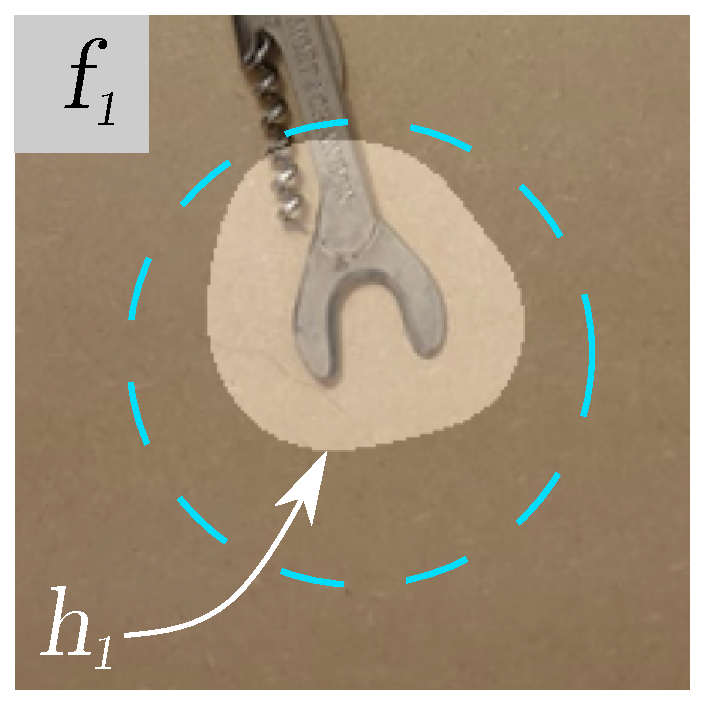
\includegraphics[width=\textwidth]{ch1-diffy/figures/fig_example/scene-h.pdf}
\caption{$f_1$ (close-up)}
\label{fig:sceneh}
    \end{subfigure}\hfil
    \begin{subfigure}{0.25\textwidth}
\includegraphics[width=\textwidth]{ch1-diffy/figures/fig_example/racoon_h.pdf}
\caption{$f_2$ (raccoon's paw)}
\label{fig:raccoonh}    \end{subfigure}\hfil
     \begin{subfigure}{0.25\textwidth}
\includegraphics[width=\textwidth]{ch1-diffy/figures/fig_example/peppers_h.pdf}
\caption{$f_3$ (pepper close-up)}
\label{fig:flowersh}
    \end{subfigure}
\smallskip
     \begin{subfigure}{0.25\textwidth}
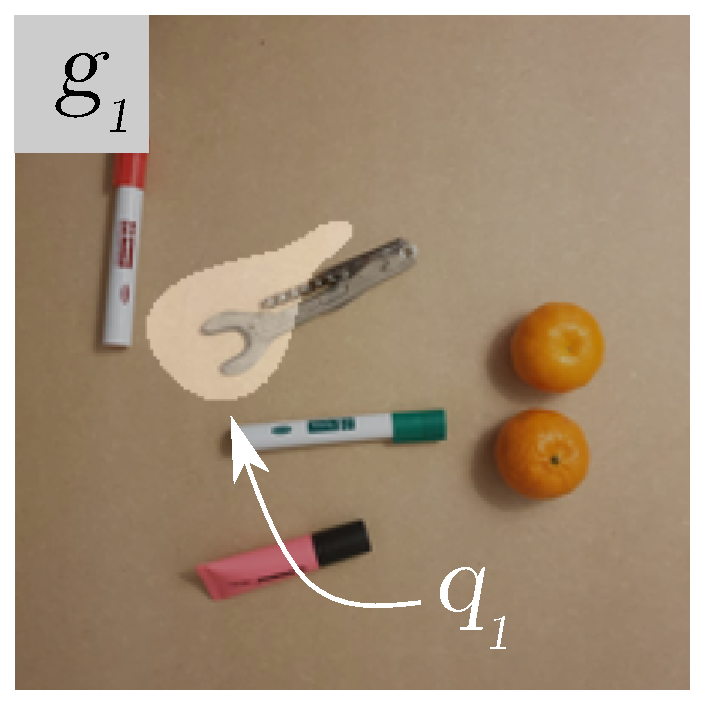
\includegraphics[width=\textwidth]{ch1-diffy/figures/fig_example/scene-q.pdf}
\caption{$g_1$ (scene with multiple objects)}
\label{fig:sceneq}
    \end{subfigure}\hfil
     \begin{subfigure}{0.25\textwidth}
\includegraphics[width=\textwidth]{ch1-diffy/figures/fig_example/racoon_q.pdf}
\caption{$g_2$ (raccoon's abdomen, with natural keystone deformation.)}
\label{fig:raccoonq}
    \end{subfigure}\hfil
     \begin{subfigure}{0.25\textwidth}
\includegraphics[width=\textwidth]{ch1-diffy/figures/fig_example/peppers_q.pdf}
\caption{$g_3$ (peppers among vegetables)}
\label{fig:flowersq}
    \end{subfigure}
\caption[Illustration of Diffy on images.]{\emph{Illustration of $\widehat D_\lambda$ on images.} We compute $\widehat D_\lambda(f_i, g_i)$ and materialize the optimal $h_i$ and $q_i$ selected by \Diffy (with thresholding for visualisation purposes), for $f_i$ and $g_i$ images taken with a smartphone. The mask $\mu$ is illustrated by the dashed circle (in light blue), see \cref{sec:details} for details. The images are taken from different views so as to provide different angles and lighting. \cref{fig:sceneh,fig:sceneq} show a scene of \texttt{objects} and a close-up on one of them (bottle opener). \cref{fig:raccoonh,fig:raccoonq} are taken from images of a raccoon (\texttt{raccoon}). \cref{fig:flowersh,fig:flowersq} are sub-patches from \texttt{peppers}, a scene with vegetables. Notice that $q_i$ visually matches the area highlighted by $h_i$, despite the perspective and scale changes. Additional details are gathered in \cref{sec:illustration}.}
\label{fig:example}
    \end{figure*}

Using tools from functional analysis, we prove that \Diffy behaves as expected when comparing $f$ and $f\circ Q$ (\emph{i.e.}, that it considers these two functions to be close) in the limit of vanishing regularization (\cref{theorem:main-theorem}). We support our theoretical claims with numerical experiments on images.

\paragraph{Outline.} We introduce our new dissimilarity in \cref{sec:dissimilarity}. In \cref{sec:robustness}, we prove that the intuition leading to the definition in \cref{sec:dissimilarity} is well founded and discuss the theoretical properties of the dissimilarity. We then show how to compute the dissimilarity in \cref{sec:computing}: we first show that it has a closed-form expression; we then present and justify an approximation scheme based on Nyström sampling. We illustrate the behavior of the dissimilarity with experiments on images in \cref{sec:experiments}.

\section{The dissimilarity}\label{sec:dissimilarity}

\subsection{Informal derivation of the dissimilarity}\label{sec:informal}

The dissimilarity we describe in this work relies on the internal structure of the objects it compares. An efficient way of encoding this structure is to, whenever possible, view objects as maps between an input space and an output space. In this way, we can consider both the values taken by the function and the locations at which these values were taken.

Consider $f$ and $g$ two maps between $\R^d$ and $\R^p$. Our goal is to determine whether there exists a diffeomorphism $Q:\R^d \to \R^d$ such that $g = f \circ Q$. In practice, such transformations could be rigid-body transformations, a non-singular projective transformation or more generally a mild distorsion of the space (such as warping). The goal is thus to find a measure of dissimilarity between $f$ and $g$ that is robust to such diffeomorphisms. We derive such a measure informally in this section around three key ideas.

\paragraph{Change of variable formula.} Integrals offer a natural way to ``eliminate'' a diffeomorphism from a function, via the change of variable formula
\eqals{
\int f(Q(x)) |\nabla Q(x)| \dd x = \int f(x) \dd x.
}
As $|\nabla Q|$ (the determinant of the Jacobian of $Q$) is unknown, we can approximate the above formula with:
\eqal{\label{eq:prob}
\min_{q} \left|\int g(x) q(x) \dd x - \int f(x) \dd x\right|,
} where $q$ lies in a space of functions.

Indeed, when $g = f\circ Q$ for some diffeomorphism $Q$, choosing $q = \vert\nabla Q\vert$ minimizes \eqref{eq:prob}. However, this solution is not unique. Indeed there exist trivial solutions as $q = f / g$, that are irrespective of the existence of a $Q$ such that $g=f\circ Q$ or not.

\paragraph{Range of statistics.} One way of reducing the class of solutions to ones that are relevant to our original question is to study not only how well the weighted integral of $g$ can approximate the integral of $f$, but also require that the same weight approximate a wide class of transformations of $f$. A natural example with inspiration in probability theory is to be able to approximate all moments of $f$, \emph{i.e.}, the integrals of the moments $v_1(f) = f, v_2(f) = f^2, \dots$, or more general statistics. The function $q = f / g$ may match the integral of $v_1(g)$ with that of $v_1(f)$, but cannot work for $v_2$. However, if $g = f\circ Q$, $q = |\nabla Q(x)|$ (the solution we are seeking), satisfies that for any continuous function $v: \R^p \to \R$,
\eqals{
\int v(f(Q(x))) |\nabla Q(x)| \dd x = \int v(f(x)) \dd x.
}
Problem \eqref{eq:prob} is thus replaced by the following one, which also has $q$ as a solution when $g = f \circ Q$:
\eqal{\label{eq:prob2}
\min_q \max_{v \in V} \left|\int v(g(x)) q(x) \dd x - \int v(f(x)) \dd x\right|,
} where $V$ is a rich set of statistics, \emph{e.g.}, continuous integrable functions on $\R^p$.

% %\begin{figure}[t]
% %    \centering
% %    \includegraphics[width=0.35\textwidth]{ch1-diffy/figures/cartoon_export.pdf}
% %    \caption{Illustration of our method. Top: $f$ image with mask $\mu$ (dashed area). Bottom: $g$ is the transformation of $f$ by a diffeomorphism $Q$. Two solutions $q_1$ and $q_2$ are illustrated. $q_1$ (blue, solid line) is obtained with regularization $\lambda_1$. $q_2$ (red, dashed line) is obtained with regularization $\lambda_2 > \lambda_1$. Notice that $q_2$ is a simpler function than $q_1$ (i.e. $\norh{q_2} < \norh{q_1}$) as \Diffy is applied with stronger regularization.}
% %    \label{fig:reg}
% %\end{figure}


\paragraph{Uniformity over regions.} Problem \eqref{eq:prob2} averages the statistics uniformly over the whole space irrespectively of the fact that a witness of $g \neq f \circ Q$ could live in a lower dimensional region. For instance $g$ and $f$ might be non-zero only on a small region of the space, consequently yielding to a relatively small value for \cref{eq:prob2}. To enhance such regions, we choose to integrate with respect to a smooth function $h$, that is chosen adversarially to maximize the dissimilarity between $f$ and $g$.  %We require that for any region of the domain of $f$ and $g$ (encoded by $h$), there exists an equally smooth function $q$ whose induced transformation on $v(g)$ matches that of $h$ on $\phi(f)$.
In other words, we arrive at the following optimization problem:
\eqals{
\max_{h \in \hh_1} \min_{q} \max_{v \in V} \left|\int v(g(x)) q(x) \dd x - \int v(f(x)) h(x) \dd x\right|,
}
where $\hh_1$ is a suitable set of smooth functions.
Again, if $g = f\circ Q$, the above is solved by $q \,=\, h\circ Q \, |\nabla Q|$.



Note that the smoothness of $h$ and $q$ is crucial. On the one hand, the smoothness of $h$ ensures that the considered regions are of interest with respect to the underlying metric on $\R^d$, i.e. they cannot be too close to diracs on pathological sets. On the other, the smoothness of $q$ ensures that the transformations are not matched by ``cherry-picking'' dispersed points on the domain such that the integrals match.


 %\begin{figure*}[ht]
 %    \centering
 %    \begin{subfigure}[b]{0.40\textwidth}
 %        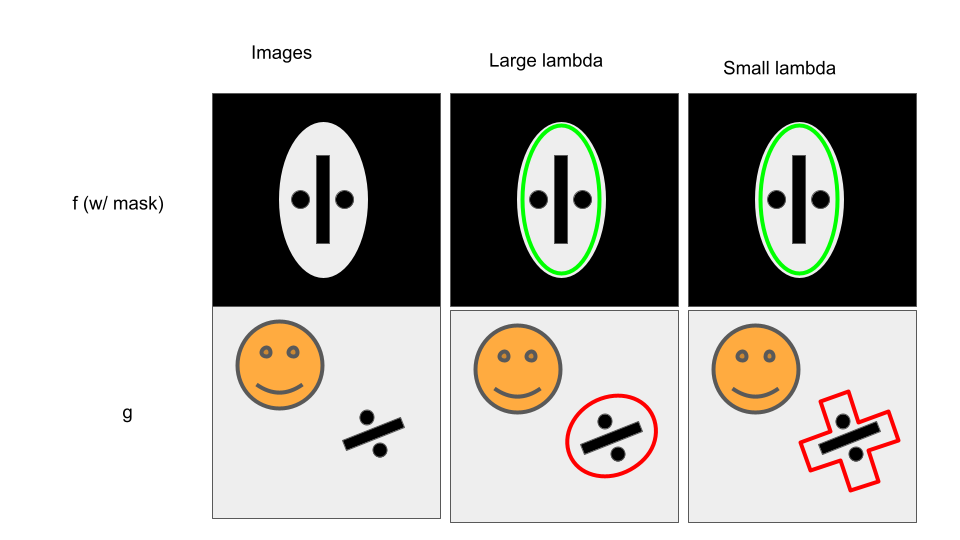
\includegraphics[width=\textwidth]{ch1-diffy/figures/sketch_reg.png}
 %        \caption{When there is a diffeomorphism: regularization ensures that the smoothest solution is found.}
 %    \end{subfigure}\quad
 %    \begin{subfigure}[b]{0.40\textwidth}
 %        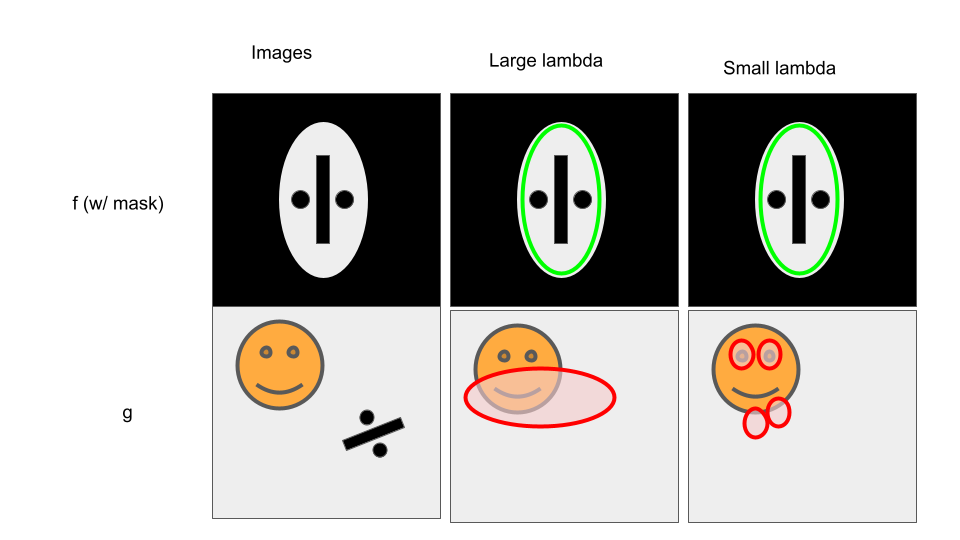
\includegraphics[width=\textwidth]{ch1-diffy/figures/sketch_reg_2.png}
 %        \caption{When there is not a diffeomorphism: regularization is essential to ensure that the distance does not try to find one at all costs!}
 %    \end{subfigure}
 %    \caption{Effect of regularization}
 %    \label{fig:reg}
 %\end{figure*}

\subsection{Definition of the dissimilarity}
Now that we have given the motivation as well as the intuition behind our method, we can formally introduce it.


Let $X \subseteq \R^d$ and $Y \subseteq \R^p$ where $d, p \geq 1$. In this paper, the objects of interest are maps from $X$ to $Y$. Note that this is quite flexible and can reflect many of the rich types of data considered in image processing, time-series modelling and machine learning. Indeed, an image can be seen as a map from $\R^2$ (the coordinates of the pixels) to $\R^3$ (the color space, RGB for instance). A time-series can be seen as a map from $\R^1$ (time) to $\R^n$ (the space of the sample values).

Let $k_X$ be a reproducing kernel on $X$ with Reproducing Kernel Hilbert Space (RKHS) $\mathcal H$  \cite{aronszajn1950theory} and $k_Y$ be a reproducing kernel on $Y$ with RKHS $\mathcal F$. In particular, we assume that they are bounded.


To conclude, the formalization below allows naturally for the presence of a mask function $\mu$, with the role of focusing the matching process on a subregion of interest of $f$. The role of the mask will be discussed after the definition.


\begin{definition}[Dissimilarity $D_\lambda(f, g)$]\label{def:D}
    Let $\la \geq 0$ and bounded integrable $\mu:\X \to \R$.  For any $f,g:X\to Y$, we define the dissimilarity
\eqal{\label{eq:def-D}
    D_\lambda(f, g) := \max_{\norh{h}\leq 1}\min_{q \in \mathcal H} \Delta_{f,g}(h, q) + \lambda \norh{q}^2
}
where $\Delta_{f, g}(h, q)$ is defined as follows,
\begin{align*}
\Delta_{f, g}(h, q) := \max_{\|v\|_{{\cal F}} \leq 1} &\Big|  \int_X v(g(x))q(x)\dd x-  \int_X v(f(x))\mu(x)h(x)\dd x\Big|^2.
\end{align*}
\end{definition}

\noindent When clear from context, we write $D$ instead of $D_\la$ for the sake of conciseness.

%The reader should easily recognize the construction described in \cref{sec:informal}. We have made the space in which we search for $q$ and $h$ precise: $\hh$, the RHKS of $k_X$. Regularity of $h$ is enforced by searching in the unit ball, while regularity of $q$ is enforced with Tikhonov regularization. This choice allows at the same time to compute the dissimilarity in closed form (see \cref{sec:computing}), while not sacrificing its expressivity (see \cref{sec:approximation}). In particular, to allow a very rich set of statistics that is also manageable from a computational viewpoint, we choose $V$ to be the unit ball of ${\mathcal F}$. For example, if $Y$ is a bounded subset of $\R^p$ and $k_Y$ is chosen as the Laplace kernel $k_Y(y,y') = \exp(-\|y-y'\|)$, then a rescaled version of any infinitely smooth function belongs to $V$ (including in particular all polynomials, smooth probabilities, Fourier basis -- see \cref{app:background} for more details). For the same reason we choose $\hh_1$ to be the unit ball of $\hh$ and we choose also $q \in \hh$.
\cref{fig:example} shows a few examples of the role played by the $h$ and $q$ optimizing the problem in \cref{eq:def-D}.


\begin{figure*}
    \centering
    \begin{subfigure}[t]{0.45\textwidth}
        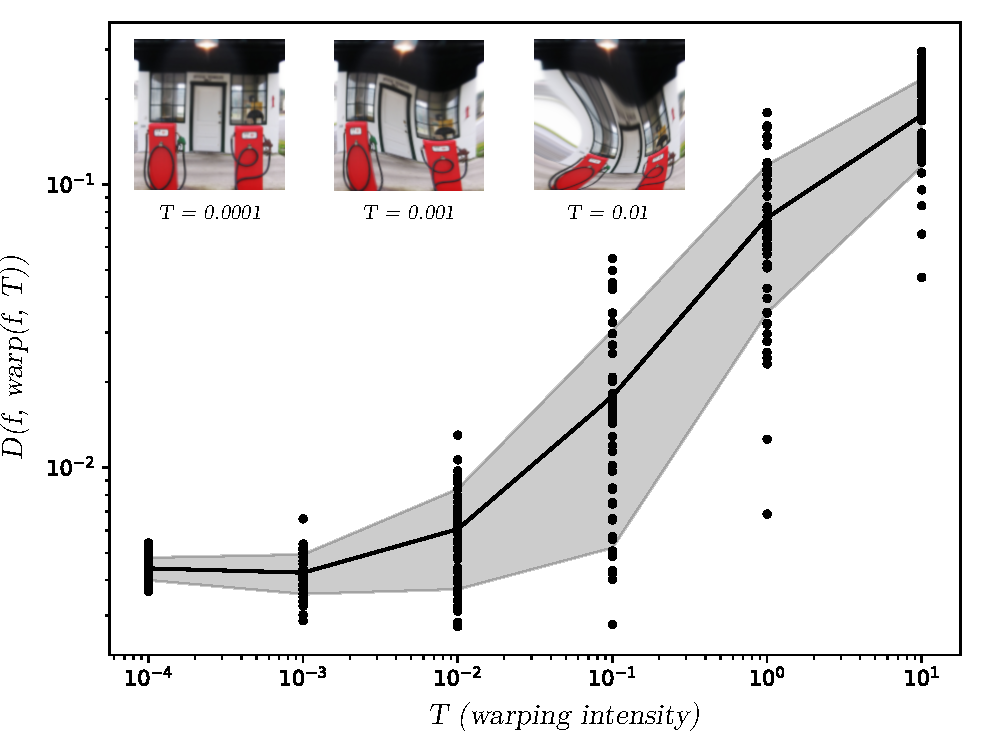
\includegraphics[width=\textwidth]{ch1-diffy/figures/fig_warping/warping_left.pdf}
        \label{fig:warping-left}
        \caption{\emph{$\widehat D_\lambda(f, \text{warp}(f, T))$ as a function of $T$.} We repeat the warp $50$ times ($+$ markers) on the same image and represent average values $\pm$ standard deviation (in grey).}
    \end{subfigure}\qquad
    \begin{subfigure}[t]{0.45\textwidth}
        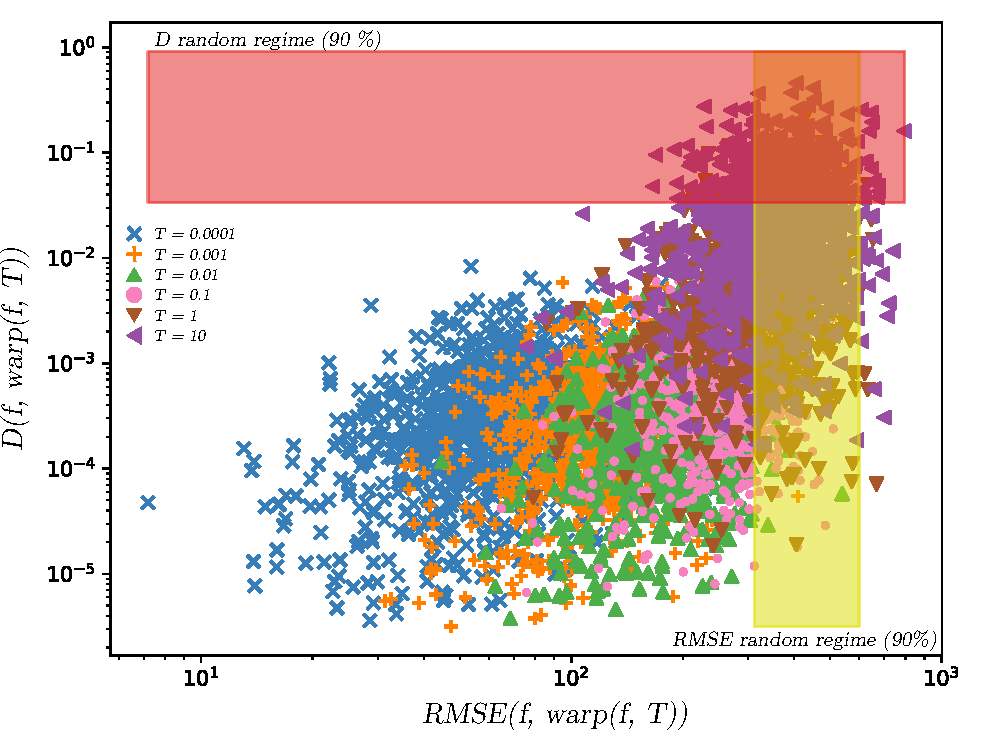
\includegraphics[width=\textwidth]{ch1-diffy/figures/fig_warping/warping_right.pdf}
        \caption{\emph{$\textrm{RMSE}(f, \textrm{warp}(f, T))$ against $\widehat D_\lambda(f, \textrm{warp}(f, T))$ for various values of $T$ and images $f$.} $1000$ images are each warped once for each value of $T$. We represent the random regime for each metric.}
    \end{subfigure}
    \caption[Invariance of Diffy to general diffeomorphisms (warping).]{\emph{Invariance to general diffeomorphisms (warping).} Warping is randomly generated, its intensity controlled by a temperature parameter $T$ (higher $T$ produces, on average, warps with higher displacement norm). In (a): $\widehat D_\la$ stays constant (i.e. invariant to the warps) as long as their norm is not too strong (small T), while RMSE increases exponentially. When $T$ becomes large the transformations become intense (indeed they are non-diffeomorphic) and $\widehat D_\la$ grows to reflect this fact.  In (b): we see that $\widehat D_\la$ stays invariant to warps as long as $T \leq 0.1$ (far from the random regime interval), while the Euclidean distance increases exponentially with $T$, even for small $T$. See \cref{sec:invariance-warping} for more details.}
    \label{fig:warping}
\end{figure*}


\paragraph{The role of the mask $\mu$.} We introduced a function $\mu:X \to \R$ which applies to the term depending on $f$ and $h$. This function is meant to be a mask which focuses the distance on a certain region of $f$, discounting other regions. Such presence is useful in practice, since typically the space $X$ is given by the problem. For example, if we want to use the dissimilarity to check if the content of a given image ($f$) is contained in an image ($g$), the shape $X$ is typically rectangular, while the region of interest is the interior of the image. In this case the mask is useful to avoid the artifacts introduced by the corners. Notice that this addition further breaks the symmetry between $f$ and $g$: $f$ becomes a \emph{reference}, and we search in $g$ for matching statistics. In the experiments, we relied for example on a Blackman Window, a classical window function in signal and image processing (see \cref{sec:details}) to reduce the impact of the corners.



%%%%%%%%%%%%%%%%%%%

\section{Robustness to diffeomorphisms}\label{sec:robustness}


The dissimilarity $D$ is designed (consistently with the derivation in \cref{sec:informal}) to be small when $f$ and $g$ are equal up to a diffeomorphism. The ideal result would be something along the lines of the following \emph{informal} theorem:

\begin{theorem}[Ideal]\label{thm:ideal}
    For any $f: X \to Y$ and any $Q$ diffeomorphism over $X$, $D(f, f\circ Q) \approx 0.$
\end{theorem}

This is of course too much to ask. Indeed, the regularization over the choice of $q$ (which in turn controls the regularity of the jacobian of a hypothetical $Q$) introduces a bias:  even if $g = f \circ Q$, the dissimilarity is not $0$. This bias vanishes if and only if $q^*=0$ (by definiteness of the norm).

However, when the RKHS is assumed to be rich enough and $Q$ and $\mu$ are regular enough, then we have the following result. Before stating it, we recall that the Laplace kernel $k_X(x,x^\prime) = \exp(-\|x-x^\prime\|)$ belongs to the more general family of Sobolev kernels \cite{wendland2004scattered}. In particular, it corresponds to the Sobolev kernel of smoothness $m$, with $m = (d+1)/2$, where $d$ is the dimension of $X \subset \R^d$.
\begin{theorem}\label{theorem:main-theorem}
Let $X \subset \R^d$ be an open bounded set with Lipschitz boundary. Let $\mu \in C^\infty(\R^d)$ with compact support $\Omega \subset X$. Choose $k_X$ to be a Sobolev kernel of smoothness $m$, with $m > d/2$. Then for any $C^{m+1}$ diffeomorphism $Q$ on $\R^d$ satisfying $Q^{-1}(\Omega) \subset X$, we have that
\eqals{
 D_\la(f, f \circ Q) ~~\leq~~ \lambda ~ C^2_{\mu} C^2_{Q} \qquad \forall f\, \textrm{measurable},
}
where $C_\mu = \|\mu\|_{H^m(\R^d)}$, and $C_Q$ is defined in \cref{eq:def-CQ} in \cref{sec:general-theorem} and depends only on $\Omega, X, Q, d, m$.
\end{theorem}
%%%%%%
The theorem above is a special case of \cref{thm:general-theorem}, presented in \cref{sec:general-theorem}. There we prove the more general result: $D_\lambda(f,g) \leq \lambda C^2_{\mu} C^2_{Q}$, for all measurable $f, g$ that satisfy $g(x) = (f \circ Q)(x)$, only in the region not canceled by the mask, \emph{i.e.}, $\forall x \in Q^{-1}(\Omega)$.



A first consequence of \cref{theorem:main-theorem} is that the regularization parameter $\lambda$ controls the threshold to decide whenever $g \approx f \circ Q$. In particular, we easily see that $D_\la(f, f \circ Q) \to 0$, when $\la \to 0$. This result confirms that in the limit where the regularization vanishes, so does the bias and we have the result we would have imagined à la \cref{thm:ideal}. We will see in \cref{sec:approximation} that $\la$ has also an important role in controlling the approximation error of $D(f,g)$. This shows that $\la$ controls a similar bias-variance trade-off as in classical kernel supervised learning \cite{shawe-taylor2004}.

To illustrate  the dependence of $C_Q$ with respect to $Q$, in the following example we explicitly compute $C_Q$ for an interesting class of diffeomorphisms.

\begin{example}[Magnitude of $C_Q$ for rigid transforms]\label{ex:diffeo}
Let $X$ be the unit ball in $\R^d$ and let $\mu$ be a mask supported on $\Omega$, the ball of radius $r < 1$. We consider the diffeomorphisms $Q(x) = \alpha R x$, with $R$ a unitary matrix and $r < \alpha < 1/r$. We use the Laplace kernel $k_X(x,x^\prime) = \exp(-\|x-x^\prime\|)$ for $k_X$ (analogously for $k_Y$).
Then, we compute explicitly the bound in \cref{eq:def-CQ}, since the Laplace kernel corresponds to Sobolev kernel with exponent $m = (d+1)/2$, obtaining
$$C_Q ~~\leq~~ C_0 \left(\frac{\alpha}{\min(\alpha,1) - r}\right)^{m+d/2}\alpha^d (1 + \alpha + \alpha^m).$$
\end{example}
\begin{remark}
By seeing data points as functions, we are able to efficiently reason about them. Hence, since data points are continuous objects, $d=\dim(X)$, the dimensions of $X$, and not the number of pixels, which we denote $N$ below. Indeed, $X$ is low-dimensional by nature: for images, $d=2$ since images are 2-d objects, while $N$ could be very large. This way, the dimensional dependence of $C_Q$ is very reasonable. In the extreme case where we consider time series of point clouds (for example, brain scans through time), $d = 4$ (time $+$ 3 spatial coordinates). If we consider a scale change range of $50\%$, then $C_Q$ is of the order of $3/2^4 \approx 5$. We emphasize that $C_Q$ is not related to the number of samples (for images, the number of pixels) used to compute DID in practice.
\end{remark}
\subsection{Discussion on the discriminatory power of $D_\la$} \label{sec:discussion-selectivity}
In \cref{theorem:main-theorem}, we proved that when $g = f \circ Q$ for some diffeomorphism $Q$, then $D(f,g)$ is small, i.e. that the dissimilarity is essentially invariant to the diffeomorphisms. However, to fully characterize the properties of the proposed dissimilarity it would be interesting to study also its discriminatory power, i.e. the fact that $D(f,g)$ is small {\em only if} there exists a diffeomorphism $Q$ such that $g = f \circ Q$. \cref{fig:warping} investigates this question from the empirical perspective. The details of these experiments are reported in \cref{sec:experiments} (and further explored in \cref{app:additional-experiments}). They show that, \Diffy is very robust to significant transformations $f\circ Q$ of the original signal $f$. Additionally we observe that $D_\la$ is very discriminative, in contrast to less diffeomorphism invariant metrics such as the euclidean distance, when comparing $D_\la(f,f\circ Q)$ with $D_\la(f,g)$ for a random signal $g$. We care to point out however, that the theoretical analysis of \Diffy's the discriminative abilities is beyond the scope of this work (whose aim is to introduce the discrepancy and study its invariance properties) and we postpone it to future research.

%%%%%% However, the experimental analysis performed in \cref{sec:experiments} and further in \cref{app:additional-experiments} strongly supports it.



%%%%%%%%%%%%%%%%%%%%%

\section{Computing the dissimilarity}\label{sec:computing}

Before deriving the closed form solution for $D_\la$, we need to recall some basic properties of kernels. Reproducing kernels and RKHSs satisfy the so called {\em reproducing property}, i.e. There exists a map $\psi:X \to \hh$ such that, for any $f \in \hh$ and $x \in X$, it holds that $f(x) = \scal{f}{\psi(x)}_\hh$, where $\scal{\cdot}{\cdot}_\hh$ is the scalar product associated to the RKHS $\hh$. Moreover $k_X(x,x^\prime) = \scal{\psi(x)}{\psi(x^\prime)}_{\hh}$, for all $x,x^\prime \in X$. The same holds for $k_Y$ and $\cal F$. i.e., there exists $\Phi:Y \to {\cal F}$ such that $v(y) = \scal{v}{\Phi(y)}_{\cal F}$ for all $v \in {\cal F}, y \in Y$ and $k_Y(y,y^\prime) = \scal{\Phi(y)}{\Phi(y^\prime)}$ for all $y,y^\prime \in Y$, where $\scal{\cdot}{\cdot}_{\cal F}$ is the inner product associated to ${\cal F}$. In particular, note that, since we assumed that $k_X, k_Y$ are bounded kernels, then there exist two constants $\kappa_X, \kappa_Y$ such that $\sup_{x \in X} \|\psi(x)\|_{\hh} \leq \kappa_X$ and analogously $\sup_{y \in Y} \|\Phi(y)\|_{\cal F} \leq \kappa_Y$.



\subsection{Closed form solution}
In \cref{def:D}, we define $D_\lambda(f,g)$ as an optimization problem in $\hh \times \hh$. In fact, this optimization problem has a closed-form solution, as the solution of an eigenvalue problem of an operator between $\hh$ and $\mathcal F$ as derived in \cref{eq:cl-form-eig-Dla}. We introduce the relevant objects and prove \cref{theorem:closed-form}.

\begin{definition}[Operators $F_\mu$, $G$]\label{def:operatorsFG}
Given $f, g: X \to Y$, the feature map $\Phi: Y\to \mathcal F$ and the mask function $\mu:X \to \R$, define the linear operators $F_\mu, G:\hh \to {\cal F}$ as follows:
\eqal{
F_\mu &= \int_X \Phi(f(x)) \otimes \psi(x) \mu(x) \dd x, \\ G~&= \int_X \Phi(g(x)) \otimes \psi(x) \dd x.
}
\end{definition}

\cref{def:operatorsFG} is a compact notation for the the integral operators in the RKHS. Noticing that we can rewrite $\Delta_{f,g}$ (see below) as a function of $F_\mu$ and $G$ is key to deriving the closed-form expression and the finite-dimensional approximation in \cref{eq:widehatA,eq:widehatB}, that can be computed in practice.

When $X$ is a bounded set, the two operators above are trace class and, by the representer property  $\scal{v}{F_\mu h}_{\cal F} = \int_X v(f(x)) h(x) \mu(x) dx$ and also $\scal{v}{G q}_{\cal F} = \int_X v(f(x)) q(x) dx$ (see \cref{lm:explicit-Fmu-G} in \cref{sec:additional-proofs} for a detailed proof). Using this result and considering the linearity of $\scal{\cdot}{\cdot}_{\cal F}$ and the variational characterization of the Hilbert norm (i.e. $\|u\|_{\cal F} = \max_{\|v\|_{\cal F} \leq 1} |\scal{v}{u}_{\cal F}|$), we have
\eqals{
\Delta_{f,g}(h,q) & = \|F_\mu h - G q\|_{\cal F}^2,
}
for any $h, q \in \hh$. From which we characterize $D_\lambda$ as
\eqal{
D_\lambda(f, g) = \max_{\norh{h}\leq 1} \min_{q\in\hh} \norf{F_\mu h - G q}^2 + \lambda \norh{q}^2.
}
To conclude, note that the optimization problem in the equation above has a closed-form expression in terms of the operatorial norm of an operator depending on $F_\mu$ and $G$. All the reasoning above is formalized below.
\begin{theorem}[Closed-form solution]\label{theorem:closed-form}
Let $X \subset \R^d$ be an open bounded set. Using the notations above, we have:
\eqal{\label{eq:cl-form-eig-Dla}
D_\lambda(f, g) = \lambda\norop{(GG^* + \lambda I)^{-1/2}F_\mu}^2.
}
\end{theorem}
The proof of \cref{theorem:closed-form} comes from identifying the inner optimization problem as a linear regression problem, and the the outer maximization problem as an eigenproblem. The complete proof is presented in \cref{sec:proof-closed-form}.

\begin{figure}[t]
    \centering
    \includegraphics[width=0.8\textwidth]{ch1-diffy/figures/fig_rotation/rotation}
    \caption[Invariance of Diffy to rotation.]{\emph{Invariance to rotation.} We consider a patch $f$ (size $100\times 100$) of a larger scene (\texttt{peppers.jpeg}) and compare it to its rotated versions $\text{rotate}(f, \alpha)$, where $\alpha$ is an angle. $D(f, \text{rotate}(f, \alpha))$ is represented with $+$ symbols and $\textrm{RMSE}(f, \text{rotate}(f, \alpha))$ with $\times$ symbols. Random regimes are represented by shaded areas (see text). Both $\widehat D_\la$ and the RMSE seem constant as a function of $\alpha$ (although with $\alpha=0$ or $\alpha=180$ a smaller value is achieved). However, the RMSE of the rotated patches falls in (or close to) the confidence interval, making them indistinguishable from random patches from the same image. $\widehat D_\la$ takes values that are over $10 \times$ smaller for rotated patches that for random patches. Hence, \Diffy is invariant to rotation, whereas RMSE is constant (for $\alpha > 0$). Here $\la = 10^{-6}$. See \cref{sec:invariance-rotation} for more details.}
    \label{fig:rotation}
\end{figure}

\section{Approximate computation}\label{sec:approximation}

Although \cref{theorem:closed-form} gives a closed-form expression of $D_\lambda(f,g)$, $F_\mu$ and $G$ are defined as integral operators between infinite dimensional Hilbert spaces. In practice, we only have access to a discretization of $f$ and $g$ (e.g. an image is a discretized spatial signal represented by $N$ pixels). A first natural approximation is thus to replace the integral with an empirical counterpart. This estimate is then a sum of rank-one operators between $\mathcal H$ and $\mathcal F$. To reduce the computational cost, while keeping good accuracy, we can then further approximate it using Nyström methods for kernels. The resulting estimator is $\widehat{D}_\la$ presented in \cref{eq:widehatD-finite-dimensional}, its convergence to $D_\la$ is studied in \cref{thm:appr-error-widehatD}.


\paragraph{Quadrature approximation.}

We replace $F_\mu$ with an estimator $F_{\mu, N}$ and $G$ with an estimator $G_N$:
\eqal{
F_{\mu, N} &= \frac{v_X}{N}\sum_{i=1}^N \Phi(f(x_i)) \otimes \psi(x_i) \mu(x_i)\label{eq:F-sum}\\
G_{N} &= \frac{v_X}{N}\sum_{i=1}^N \Phi(g(x_i)) \otimes \psi(x_i),\label{eq:G-sum}
}
where $v_X := \int_X \dd x$ is the volume of the domain $X$.
Note that the set of $\lbrace x_1, \ldots, x_N \rbrace$ can be chosen at random or arbitrarily to best approximate the integrals. $F$ and $G$ can be approximated using different points. In practice, they are often given as the positions of pixels of images, sample times of a time series.

\paragraph{Nyström approximation.}

From the previous section, it is clear that $\rank{F_{\mu, N}} \leq N$ and $\rank{G_N} \leq N$. This justifies using the low-rank approximations we introduce in this section. It is possible to further reduce the rank of the matrices, while keeping a good accuracy, by using the so-called {\em Nystr\"om approximation} \cite{williams2001using,drineas2005nystrom,rudi2015less}.

Let $M_X, M_Y \in \N$ and choose the set of points $\widetilde{X} = \lbrace \widetilde x_1, \ldots, \widetilde x_{M_X}\rbrace \subset X$ and $\widetilde{Y} = \lbrace \widetilde y_1, \ldots, \widetilde y_{M_Y} \} \subset Y$. The Nystr\"om approximation of a vector $v \in \hh$ is the projected vector $P_{\tilde{X}} v$, where $P_{\tilde{X}} :\hh \to \hh$ is the projection operator with range corresponding to $\textrm{span} \{\psi(\tilde{x}_1),\dots,\psi(\tilde{x}_{M_X})\}$. Note, in particular, that $P_{\tilde{X}}$ has rank $M_X$ when $k_X$ is universal. $P_{\tilde{Y}}: {\cal F} \to {\cal F}$ on $\tilde{Y}$ in defined analogously.


\paragraph{Combining the two approximations.}
Assume in this section, that the kernels of choice are universal (as, e.g., the Laplacian or the Gaussian kernel).
Let $P_{\tilde{X}}:\hh \to \hh$ be the projection operator associated to the Nystr\"om points on $X$ and $P_{\tilde{Y}}$ the one associated to the Nystr\"om point on $Y$. Combining the two approximations, we define the following estimator for $D_\la$,
\eqals{
\widehat{D}_\la(f,g) := \la \|(P_{\tilde{Y}} G_N P_{\tilde{X}} G_N^*P_{\tilde{Y}} + \la)^{-\frac{1}{2}} P_{\tilde{Y}} F_{\mu, N} P_{\tilde{X}} \|^2_{\mathrm{op}}.
}
Note, however, that $\widehat{D}_\la(f,g)$ has a finite dimensional characterization that we are going to derive now.
Let $K_{\widetilde Y f} \in \mathbb R^{M_Y \times N}$ the matrix defined by $(K_{\widetilde Y f})_{i, j} = k_Y(\widetilde y_i, f(x_j))$, $K_{\widetilde Y g}$ in an analogous way, and finally, $K_{X \widetilde X}\in\R^{N \times M_X}$ the matrix defined by $(K_{X\widetilde X})_{i, j} = K_X(x_i, \widetilde x_j)$. Let $\widehat \mu = \left[ \mu(x_1), \ldots, \mu(x_{M_X})\right]$ and $R_{\widetilde X} \in\R^{M_X \times M_X}$ be the upper-triangular Cholesky decomposition of $K_{\widetilde X \widetilde X}$ defined by $(K_{\widetilde X \widetilde X})_{ij} = k_X(\widetilde x_i, \widetilde x_j)$. Analogously, define $K_{\widetilde Y \widetilde Y}$ and define $R_{\widetilde Y}\in\R^{M_Y \times M_Y}$ its Cholesky decomposition. Note that the decomposition exists since the kernel $k_X$ is universal and so the kernel matrix $K_{\tilde{X},\tilde{X}}$ is invertible.


We introduce the following operators $\widehat{A}, \widehat{B} \in \R^{M_Y \times M_X}$, which are the finite dimensional representations in appropriate spaces $\R^{M_X}, \R^{M_Y}$ of, respectively, $\tilde{P}_Y F_{\mu, N} \tilde{P}_X$ and $\tilde{P}_Y G_N \tilde{P}_X$:
\eqal{
\widehat{A} ~&=~ \frac{v_X}{N} R_{\widetilde Y}^{-T} K_{\widetilde Y f} \diag{\widehat \mu} K_{X\widetilde X} R_{\widetilde X}^{-1},\label{eq:widehatA}\\
\widehat{B} ~&=~ \frac{v_X}{N} R_{\widetilde Y}^{-T} K_{\widetilde Y g} K_{X\widetilde X} R_{\widetilde X}^{-1}. \label{eq:widehatB}
}
In particular, we have the following characterization for $\widehat{D}_\la$.
\begin{lemma}\label{lm:widehatD}
With the notation above,
\eqal{\label{eq:widehatD-finite-dimensional}
\widehat{D}_\la(f,g) = \la \|\widehat{A}^* (\widehat{B} \widehat{B}^* + \la I)^{-1} \widehat{A}\|_{\mathrm{op}}.
}
\end{lemma}

Note that, in practice, $\widetilde X$ and $\widetilde Y$ can be chosen either deterministically, e.g. on a grid, or randomly. Now, we provide a bound on the approximation error associated to $\widehat{D}_\la(f,g)$. We assume that the $N$ points in $x_1,\dots, x_N$ are sampled independently and uniformly at random in $X$ and, moreover, that the $M_X$ points in $\widetilde{X}$ and the $M_Y$ points in $\widetilde{Y}$ are sampled independently and uniformly at random in, respectively, $X, Y$ (similar result can be derived for a grid).
\begin{theorem}\label{thm:appr-error-widehatD}
Let $\delta \in (0,1)$. Let $X \subset \R^d, Y \subset \R^p$ be bounded sets and $k_X, k_Y$ be Sobolev kernels with smoothness, respectively, $s + d/2$ and $z+p/2$, for some $s,z > 0$. There exists two constants $c_1, c_2$ s. t., when $M_X \geq c_1$ and $M_Y \geq c_2$, then the following holds with probability $1-\delta$,
$$|\widehat{D}_\la(f,g) - D_\la(f,g)| \leq c\left(\tfrac{\log\frac{1}{\delta}}{\la\sqrt{N}} + \tfrac{\left(\log \frac{M_X}{\delta}\right)^{\alpha}}{\la M_X^{s/d}} + \tfrac{\left(\log\frac{M_Y}{\delta}\right)^{\beta}}{\la M_Y^{z/p}}\right),$$
for any measurable $f,g : X \to Y$, where $\widehat{D}_\la(f,g)$ is defined as in \cref{eq:widehatD-finite-dimensional}. Here $c_1, c_2, c$ depend only on $X, Y, \mu, s, z, d, p$, while $\alpha = s/d+1/2$, $\beta = z/p+1/2$.
\end{theorem}

The theorem above shows that the estimation error of $\widehat{D}_\la$ with respect to $D_\la$ goes to $0$ when $N, M_X, M_Y \to \infty$. On the contrary, the error diverges in $\la$. This is in accordance with the fact that the error is of variance type and shows that $\la$ plays the role of a regularization parameter. The bound shows also that, when $s \gg d$ and $z \gg p$, i.e. when we are choosing very smooth Sobolev kernels, the decay rate of the error in $M_X$ and $M_Y$ is faster. For example, if we choose $s = r d$, $z = r p$, for some $r > 0$, then choosing $M_X = M_Y =  O(N^{r/2})$ leads to the rate
$$ |\widehat{D}_\la(f,g) - D_\la(f,g)| = O\left(\frac{1}{\la \sqrt{N}}\right).$$

\paragraph{On the choice of $\la$.}
To conclude, a choice of $\la$ as $\la = N^{-1/4}$ guarantees a final convergence rate of $\widehat{D}_\la$ to $D_\la$ in the order of $N^{-1/4}$ and, together with \cref{theorem:main-theorem} a level of invariance to diffeomorphism for $\widehat{D}_\la$ of the order
$$\widehat{D}_\la(f, f \circ Q) = O(N^{-1/4} C_\mu^2 C_Q^2),$$
which can become a statistically significant threshold to decide if, in practice $f \approx g$ up to diffeomorphism.
Clearly the choice of $r,s$ while reducing the number of Nystr\"om points required in the approximation (with important computational implications that we see below) increases the constant $C_Q$ as shown, e.g., in \cref{ex:diffeo}, where $m = s + d/2$.


%%%%%{\color{red}\bf[Algorithm?]}

\paragraph{Algorithm and computational complexity.}
The final form of the empirical estimator $\widehat{D}_\la$ is \cref{eq:widehatD-finite-dimensional}. An efficient algorithm to compute it is, for instance, (1) first computing the matrices $\widehat{A}$ and $\widehat{B}$, then the inverse $\widehat{C} = (\widehat{B}\widehat{B}^* + \la)^{-1}$ and finally compute the largest eigenvalue of $\widehat{A}^* \widehat{C} \widehat{A}$ via a power iteration method \cite{trefethen1997numerical}. %that is a method based on matrix vector products. In particular this last step avoids to compute explicitly the product of the three matrices, $\widehat{A}^* \widehat{C} \widehat{A} v = \widehat{A}^* (\widehat{C} (\widehat{A} v))$.

Assuming that (a) the cost of one kernel computation in $\R^d$ is $O(d)$ (as in the case of any translation invariant kernel as the Laplace kernel) (b) $M_X \leq N$ and $M_Y \leq N$ (which is reasonable in light of \cref{thm:appr-error-widehatD}), then the cost of computing $\widehat{D}_\la$ with the algorithm above is
$O(d N M_X + p N M_Y + M_XM_Y^2 + M_X^3 + M_Y^3)$.
Choosing the parameters, as in the discussion after \cref{thm:appr-error-widehatD}, with $r = 1$, would lead to a total computational cost of
$O(N^{3/2}(p+d)).$

Computing \Diffy between different pairs of data-points can easily be parallelized as each computation relies on matrix-vector products and matrix inversions.

\paragraph{Choice of kernel hyperparameters.}
As in any kernel-based method, selecting kernel hyper-parameters is important. The usual considerations apply: we advise cross-validation should be used to choose hyper-parameters (such as the bandwith). We do not discuss this further for space considerations.

In the theoretical analysis above, the rates in $N$ hold for any parameter of the kernel, but constants depend on the chosen parameters. This is typical of the Sobolev analysis technique, where the important parameter is the kernel regularity $m$, which corresponds to the differentiability class of the diffeormorphisms one aims to capture.

Finally, the method introduced is empirically quite robust to the choice of parameters.

 %Here we study an efficient strategy to compute it and its computational complexity. Denote $T(d)$ the cost of one kernel evaluation between two points in $\R^d$ (e.g. for the Laplace kernel $T(d) = O(d)$).

 %\textbf{Offline pre-computation~}

 %$R_{\widetilde X}$ is constructed by first computing $K_{\widetilde X\widetilde X}$ in $O(T(d)M_X^2)$ time, then a Cholesky decomposition computation in $O(M_X^3)$ time, for a total ost of $O(T(d)M_X^2 + M_X^3)$. Similarly, computing $R_{\widetilde Y}$ costs $O(T(p)M_Y^2 + M_Y^3)$.  Finally, computing $K_{X\widetilde X}$ costs $O(T(d)M_XN)$.

 %Thus, the computations that can be done offline cost: $O(T(d)M_X(M_X + N) + T(p)M_Y^2 + M_X^3 + M_Y^3)$.

\begin{figure}[t]
    \centering
    \includegraphics[width=0.8\textwidth]{ch1-diffy/figures/fig_regularization/regularization.pdf}
    \caption[Effect of regularization on Diffy.]{\emph{Effect of regularization.} We consider the same image and setting as in \cref{fig:warping} and vary $T$ and $\lambda$ (shaded areas are std deviation over $50$ warps). Observe: (1) $\widehat D_\la$ increases as a function of $T$ (as the norm of the diffeomorphism increases); (2) $\widehat D_\la$ is  proportional to $\lambda$. Both of these phenomena are predicted by \cref{theorem:main-theorem}. See \cref{sec:regularization} for more details.}
    \label{fig:regularization}
\end{figure}


 %$\widehat F$ (and $\widehat G$) can be computed in  $O(M_Y^2 N + NM_XM_Y + M_YM_X^2)$ time. This assumes that the computation is done from right to left. If it is done from left to right, then it becomes $O(M_X^2N + N M_XM_Y + M_XM_Y^2)$, which reduces the complexity in $M_Y$. Depending on the application, $M_X$ or $M_Y$ can tend to be larger and in this case one of the orders is advantageous.

 %The inverse of $\widehat G \widehat G^* + \lambda I$ is computed in $O(M_X^3)$ time, and its product with $\widehat F_\mu$ and $\widehat F_\mu^*$ is $O(M_X^2M_Y + M_Y^2M_X)$.


 %Finally, using a power iteration algorithm
 %\cite{trefethen1997numerical} to compute the operator norm of the computed $M_X \times M_X$ matrix is (naïvely) in $O(kM_X^3)$, where the algorithm does $k$ iterations. If $M_Y \ll M_X$ then we can permute terms in the operator norm and reduce the computation to $O(kM_Y^3)$.

 %In the online phase of the algorithm, that is when we compute $\widehat D_\lambda(f, g)$ for many pairs $(f, g)$, the complexity is of order $O(NM_XM_Y + N\max(M_X, M_Y)^2)$. As we hinted above, this complexity can be reduced by adapting the order of operations and the computation to the problem, i.e. to the relative sizes of $M_X$, $M_Y$ and $N$.



%%%%%%%%%%%%%%%


\section{Experiments}\label{sec:experiments}

This section investigates the empirical performance of \Diffy. We observe that, in line with our results in \cref{theorem:main-theorem}, when $g=f\circ Q$ the resulting $D_\la$ is small, while it is consistently large for signals that are not diffeomorphic versions of $f$.


\subsection{Implementation details}\label{sec:details}

We implemented $\widehat{D}_\la$ as in \cref{eq:widehatD-finite-dimensional} as described in the end of \cref{sec:approximation} using standard linear algebra routines such as matrix and matrix-vector products, matrix inversions, and eigendecompositions. The Python source code used for the experiments presented here is freely available at \href{https://github.com/theophilec/diffy}{https://github.com/theophilec/diffy}, depends on Numpy and Pytorch and supports using GPUs.

\paragraph{Normalization.}
In practice we normalize $\widehat A$ and $\widehat B$ by their operator norms $\norop{\widehat A}$ and $\norop{\widehat B}$. This normalizes $D_\lambda$ between $0$ and $1$ and makes interpretation easier.

\paragraph{Choice of mask.}
We choose $\mu$ to be a Blackman window, a standard windowing function in image processing. In 1-D, the Blackman window is defined for any $0 \leq t \leq 1$ as:
$\mu(t) = 0.42 - 0.5\cos(2\pi t) + 0.08 \cos(4\pi t)$ \cite{oppenheim99}.
We generalize it to higher-dimension by considering its tensor-product over dimensions.

\paragraph{Choice of kernel.}
Because we work with images in the experiments we present, $X = \R^2$ (coordinate space) and $Y = \R^3$ (color space). We consider the Gaussian kernel defined as $k(x, x^\prime) = \exp(- \|x - x^\prime\|^2/(2\sigma^2))$ on $X$ and the Laplace kernel defined as $k(y, y^\prime) = \exp(-a \| y - y^\prime \|)$ on $Y$. For the experiments presented in this paper, unless otherwise stated, \Diffy has parameters: $M_X = 100$, $M_Y = 16^3$, $\sigma = 1/6$ and $a=5$.

\paragraph{Datasets.}
We rely on images from Imagenet (more precisely from the \texttt{Imagenette} subset), example images from the Matlab software (\texttt{peppers}), and finally images taken with our personal devices for illustrations (\texttt{raccoon, flowers, objects}). All images are made available with the source code.

\paragraph{Diffeomorphism generation.} Diffeomorphism are obtained either by affine transformations or by generating warpings. In particular, for warpings, we use the code from \cite{wyartdiffeo}. We generate random transformations of images by displacing each of its coordinates independently (while enforcing zero displacement at the edge of the grid) then interpolating the colors.  We choose the standard deviation of the displacements of each pixel so as to obtain a transformation of given (average) displacement norm. This can be controlled by two parameters $T$ (a temperature, between $10^{-4}$ and $10^1$) and $c$ (a cut-off parameter, taking $c=2$). We denote $\text{warp}(f, T)$ such a (random) warp. Examples of warps for various $T$ parameters (and samples) are provided in \cref{sec:appendix-warping}.

\subsection{Illustrative examples}\label{sec:illustration}

In \cref{fig:example}, we show how the $h$ and $q$ that optimize \Diffy concentrate on related regions on for different scenes which which are related by a diffeomorphism, in particular rigid-body and perspective for \texttt{objects} and keystone deformation for \texttt{raccoon}. We present supplementary illustrative examples in \cref{app:additional-experiments}.

\subsection{Invariance to warping}\label{sec:invariance-warping}
Diffeomorphisms (even infinitely regular) are a much wider class of transformations than rigid body transformations such as scale, rotation and translation (or combinations thereof). In this experiment (\cref{fig:warping}), we evaluating \Diffy's behavior against a wide family of transformations (we call warps). Consider $f$ an image from $\texttt{Imagenette}$. For $T = 10^{k}$ for $-4 \leq k \leq 2$ and various images, we evaluate $\widehat D_\lambda(f, \text{warp}(f, T))$ as well as $\textrm{RMSE}(f, \text{warp}(f, T))$. We compare the values observed to $\widehat D_\la(f, g)$ and $\textrm{RMSE}(f, g)$ for random images $f$ and $g$. We call this the \emph{random regime} ($90\%$ confidence interval). Finally, we look at the performance of \Diffy on a fixed image (gas station), with repeating warps. \cref{fig:warping} shows that \Diffy is invariant to diffeomorphic warping for $T \leq 10^{-1}$ whereas the Euclidean distance increases exponentially with $T$ (making $\text{warp}(f, T)$ indistinguishable from $g$, a random image).

\subsection{Invariance to rotation}\label{sec:invariance-rotation}
The \texttt{peppers} image is often used to demonstrate image registration techniques. In this experiment (see \cref{fig:rotation}) we show that \Diffy is invariant to rotation using patches taken from it. Consider $f$ a patch from \texttt{peppers} and $g = \text{rotate}(f, \alpha)$, rotated version of $f$ by angle $\alpha$ (in practice, we rotate a larger patch then crop to avoid artifacts). We then compare $D(f, \text{rotate}(f, \alpha))$ and $\textrm{RMSE}(f, \text{rotate}(f, \alpha))$. We show that while the Euclidean distance is \emph{constant} for $\alpha \neq 0$, \Diffy is \emph{invariant}. We compare \Diffy's and the Euclidean distance values with their values for random patches from the image. As before, we call this the \emph{random regime} ($90\%$ confidence interval). This shows that the Euclidean distance is not able to distinguish between a random patch and a rotated version of the same patch, while \Diffy can. See \cref{fig:rotation} for the results of the experiments.

\subsection{Effect of regularization}\label{sec:regularization}
In order to understand the effect of regularization, we reuse the setup from \cref{sec:invariance-warping} with a single image, with varying $\lambda$. In \cref{fig:regularization}, we observe two phenomena: (1) as $T$ increases, so does $D$; (2) as $\lambda$ decreases, so does $D$. This shows that \Diffy behaves close to what is predicted by \cref{theorem:main-theorem}. Indeed, $D$ seems proportional to $\lambda$. Also, as $T$ increases, so does the norm of the transformation between $f$ and $\text{warp}(f, T)$. This makes the upper bound of \cref{theorem:main-theorem} increase in turn.
